%!TEX root = ../Thesis.tex

\chapter{Konzeption des Spurerkennungs-Moduls}
\label{cha:konzeption}

In diesem Kapitel wird das zu entwickelnde Teilmodul \textit{``Spurerkennung''}
der Anwendung \textit{Vehicle-Tracker} konzipiert. Hierzu wird zuerst dessen Rolle und Position im Gesamtkontext
der Anwendung betrachtet. Anschließend werden die Anforderungen und ein grober Entwurf des Moduls vorgestellt.

\section{Überblick über das Gesamtsystem}

Das Modul \textit{Spurerkennung} dient der Erreichung der in Abschnitt
\ref{sec:motivation_goals} definierten Ziele. Erstellt wird es im Rahmen des MEC-View Teilprojektes
\textit{Luftbeobachtung} als Teilmodul der Anwendung \textit{Vehicle-Tracker}.
Abbildung \ref{fig:concept_laneDetection_context} gibt einen Überblick über das System.
Es werden hierbei jene Module beziehungsweise Schritte vorgestellt, welche mit der Spurerkennung in
Zusammenhang stehen.

\begin{figure}[H]
    \centering
    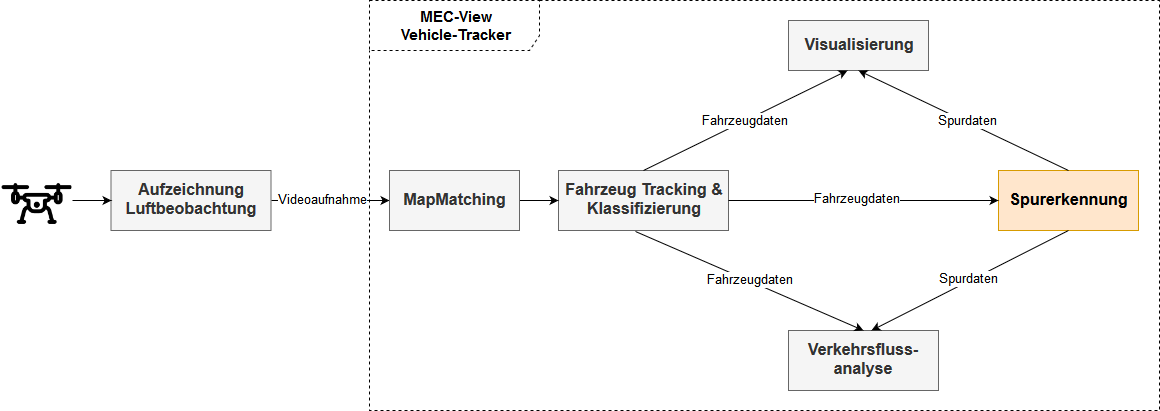
\includegraphics[width=\linewidth]{resources/img/konzeption/Context_LaneDetection}
    \caption{Kontext des Moduls Spurerkennung}
    \label{fig:concept_laneDetection_context}
\end{figure}

Die mithilfe von Drohnen erstellten Videoaufnahmen können in der MEC-View \textit{Vehicle-Tracker} Applikation
verarbeitet und analysiert werden. In einem ersten Schritt namens \textit{``MapMatching''} wird für eine Aufnahme
ein Weltkoordinatensystem in Metern definiert. Anschließend werden die Positionen
der Fahrzeuge bestimmt. Diese ersten zwei Schritte sind in Kapitel \ref{sec:position_extraction} genauer beschrieben.
Die Fahrzeuginformationen, insbesondere die Positionsinformationen, dienen dem \textit{Spurerkennung}-Modul
als Eingabe. Aus ihnen extrahierte Spurdaten können anschließend in der Anwendung visualisiert werden oder in Kombination
mit den Fahrzeuginformationen zur Analyse des Verkehrsflusses eingesetzt werden.


\section{Anforderungen an die Spurerkennung}
\label{sec:requirements}

In diesem Abschnitt werden die wichtigsten funktionalen und nicht funktionalen Anforderungen
an das Modul Spurerkennung festgehalten.

\subsection{Funktionale Anforderungen}

\paragraph{Anforderung 1000 (Top-Level)}
Das \textit{Spurerkennungs}-Modul soll es ermöglichen, mithilfe der Anwendung \textit{Vehicle-Tracker},
automatisch Fahrspuren in Luftaufnahmen anhand von Trajektoriedaten zu erkennen.

\paragraph{Anforderung 2000}
Das Modul soll die Erkennung von Fahrspuren in den folgenden Straßentopologien unterstützen:

\begin{itemize}
    \item Gerade Fahrbahnen (Landstraßen, Autobahnen, et cetera)
    \item Kreuzungen
    \item Kreisverkehre
    \item Sich öffnende oder schließende Spuren (z.B. Be- oder Entschleunigungsstreifen)
\end{itemize}

\paragraph{Anforderung 2100}
Das Modul soll unabhängig vom Aufnahmewinkel der Kamera Fahrspuren zuverlässig aus Videoaufnahmen ableiten können.

\paragraph{Anforderung 2200}
Das Modul soll Fahrspuren bei Überlagerungen sinnvoll partitionieren können.

\paragraph{Anforderung 2300}
Die von dem Modul ermittelten Fahrspuren sollen so genau wie möglich mit den realen Fahrspurverläufen auf der Straße übereinstimmen.

\paragraph{Anforderung 2400}
Das Modul soll die Enden benachbarter und paralleler Fahrspuren aneinander angleichen.

\paragraph{Anforderung 2500}
Das Modul soll es ermöglichen, die aus den Trajektorien abgeleiteten Fahrspuren in der Anwendung \textit{Vehicle-Tracker}
zu visualisieren.

\subsection{Nicht funktionale Anforderungen}

\paragraph{Anforderung 3000}
Das \textit{Spurerkennungs}-Modul muss möglichst robust mit Ausreißern und Defekten in den Trajektorien umgehen können.

\paragraph{Anforderung 3100}
Die Performance des Spurerkennung-Vorgangs ist nicht von höchster Priorität. Eine Erkennung soll allerdings
dennoch maximal wenige Minuten dauern.

\section{Entwurf des Moduls}
\label{sec:design}

In diesem Abschnitt wird, basierend auf den Erkenntnissen der Literaturrecherche und den Anforderungen,
ein grober Entwurf des \textit{Spurerkennung}-Moduls vorgestellt.

Das Modul enthält einen Algorithmus, welcher aus Fahrzeugtrajektorien Fahrspuren ableitet.
Die Grundfunktionsweise dieses Algorithmus ist in Abbildung \ref{fig:concept_laneDetection_activity}
in Form eines Aktivitätsdiagrams dargestellt.

\begin{figure}[H]
    \centering
    \includegraphics[width=0.8\linewidth]{resources/img/konzeption/activity_laneDetection}
    \caption{Basis-Ablauf des Spurerkennungsalgorithmus}
    \label{fig:concept_laneDetection_activity}
\end{figure}

Die einzelnen Schritte des Algorithmus werden im \textit{Spurerkennungs}-Modul als einzelne Komponenten
implementiert.
Die \textit{Vehicle-Tracker} Applikation ist in Java und Scala implementiert. Ihre Benutzeroberfläche basiert
auf JavaFX. Das in dieser Arbeit erstellte Modul wird komplett mit Scala umgesetzt.